\subsubsection{Qualification}
We prepared 10 qualification questions; all are yes/no questions.
We used the qualification test to train turkers to understand the requirements better. 
Each question had a hint that stated which requirement and examples were helpful for solving the question. The purpose of the qualification test was not to trick annotators but to ensure speed and quality of the annotation. 
We show one question from the qualification in Figure \ref{v2.qualification.1}. 
To see the full test, refer to: \url{https://erinzhang1998.github.io/portfolio/v2qual}. 
At the end, we recruited 88 annotators to work on our task. 

\begin{figure*}[!h]
\centering
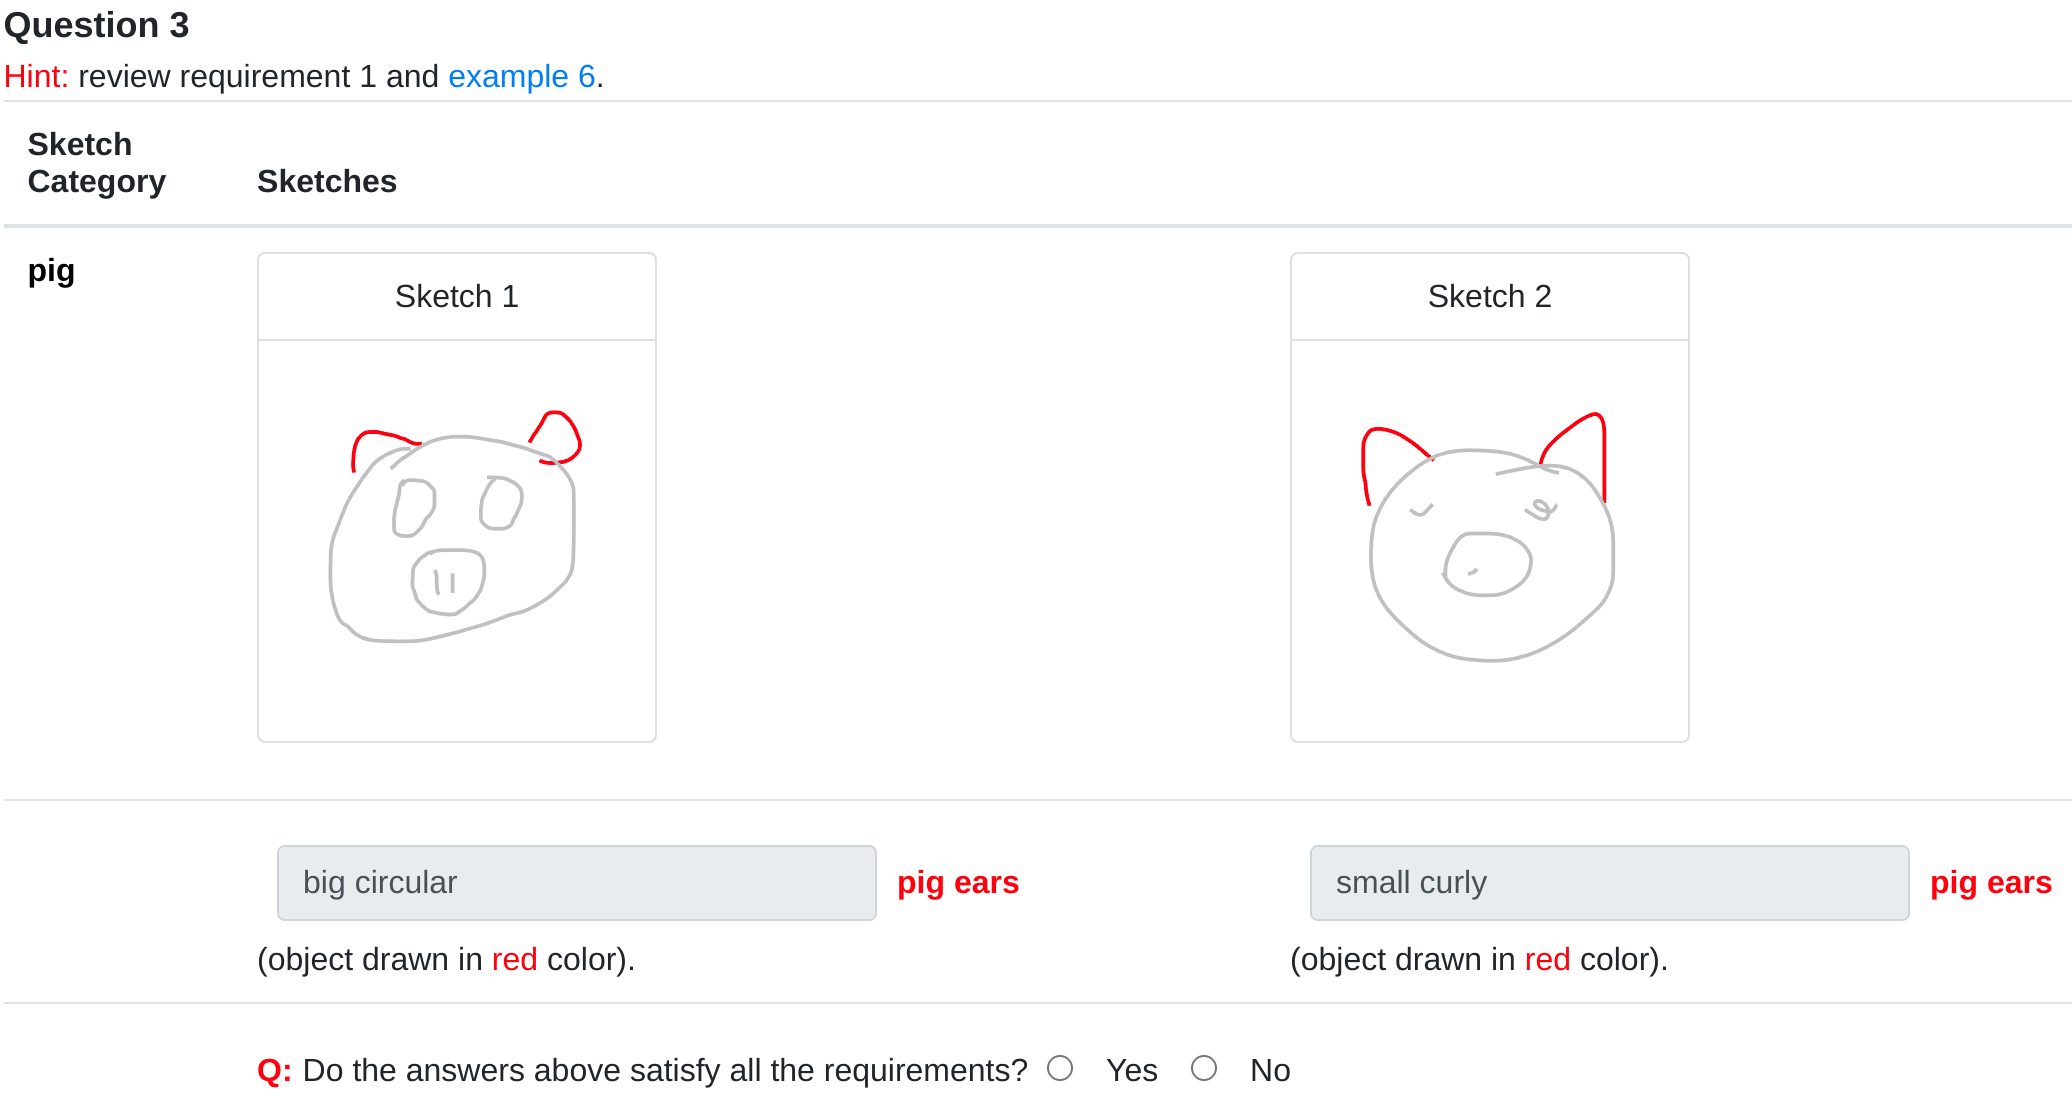
\includegraphics[width=\linewidth]{data_collection/version2/v2qualQ3.png}  
\caption{Question 3 from the qualification test used to collect the contrasting sketch text dataset (Section \ref{datav2}). We show a hint at the beginning of each question telling the annotators which requirement this question is testing. In this way, we encourage them to review the requirements to have a good understanding of the task and can then provide high-quality annotations in the real HIT. The question interface is the same as the main task interface that annotators will see when they annotate. The 1-to-1 mock-up helps them to be familiar with the workflow.}
\label{v2.qualification.1}
\end{figure*}

% \begin{table*}[!htb]
% \begin{minipage}[b]{1\textwidth}
% \centering
% \begin{tabular}{l|rrrrrrrrrr}
% \toprule
% Question Number  & 1 & 2 & 2 & 2 & 2 & 2 & 2 & 2 & 2 & 2  \\
% Correct Rate  & 1 & 2 & 2 & 2 & 2 & 2 & 2 & 2 & 2 & 2\\
% \bottomrule
% \end{tabular}
% \caption{Success rate of each question in the qualification test}
% \label{v2.qualification.success_rate}
% \end{minipage}
% \end{table*}
% We released $n$ copies of qualifications, and $n_2$ annotators scored $90$ or higher. The average score for the entire test is $x$, and the rate of correct answer for each question is shown in Table \ref{v2.qualification.success_rate}. Before releasing the qualification, we have tested the test on 
